% Created 2020-03-03 Tue 20:53
% Intended LaTeX compiler: pdflatex
\documentclass[unicode, 12pt, aspectratio=43]{beamer}
\usepackage[utf8]{inputenc}
\usepackage[T1]{fontenc}
\usepackage{graphicx}
\usepackage{grffile}
\usepackage{longtable}
\usepackage{wrapfig}
\usepackage{rotating}
\usepackage[normalem]{ulem}
\usepackage{amsmath}
\usepackage{textcomp}
\usepackage{amssymb}
\usepackage{capt-of}
\usepackage{hyperref}
\usetheme{Madrid}
\usefonttheme{professionalfonts}
\usepackage[T1]{fontenc}
\usepackage[sort, compress]{natbib}
\let\realcitep\citep \renewcommand*{\citep}[1]{{\footnotesize\realcitep{#1}}}
\usepackage{url}
\setbeamertemplate{footline}{ \hfill \usebeamercolor[fg]{page number in head/foot} \usebeamerfont{page number in head/foot} \insertframenumber\kern1em\vskip2pt }
\setbeamertemplate{itemize item}{\small\raise0.5pt\hbox{$\bullet$}}
\setbeamertemplate{itemize subitem}{\tiny\raise1.5pt\hbox{$\blacktriangleright$}}
\setbeamertemplate{navigation symbols}{}
\usepackage{xltxtra}
\usepackage{pgfpages}
\XeTeXlinebreaklocale "ja"
\setsansfont{Noto Sans CJK JP}
\usetheme{default}
\author{愛媛大 M1 出口 祥之 \\ \small{e-mail: <\texttt{deguchi@ai.cs.ehime-u.ac.jp}>}}
\date{第 1 回 NAT 勉強会: 2020/03/05}
\title{Fast Structured Decoding \\ for Sequence Models}
\subtitle{(Sun et al., NeurIPS 2019)}
\hypersetup{
 pdfauthor={愛媛大 M1 出口 祥之 \\ \small{e-mail: <\texttt{deguchi@ai.cs.ehime-u.ac.jp}>}},
 pdftitle={Fast Structured Decoding \\ for Sequence Models},
 pdfkeywords={},
 pdfsubject={},
 pdfcreator={Emacs 26.3 (Org mode 9.1.9)}, 
 pdflang={English}}
\begin{document}

\maketitle

\begin{frame}[label={sec:org085a8f9}]{Links}
\begin{itemize}
\item Fast Structured Decoding for Sequence Models (Sun et al, NeurIPS 2019)
\begin{itemize}
\item \href{https://papers.nips.cc/paper/8566-fast-structured-decoding-for-sequence-models}{\url{https://papers.nips.cc/paper/8566-fast-structured-decoding-for-sequence-models}}
\end{itemize}

\item ソースコード (Fairseq)
\begin{itemize}
\item \href{https://github.com/pytorch/fairseq/blob/master/fairseq/models/nat/nat\_crf\_transformer.py}{\url{nat_crf_transformer.py}}
\item \href{https://github.com/pytorch/fairseq/blob/master/fairseq/modules/dynamic\_crf\_layer.py}{\url{dynamic_crf_layer.py}}
\end{itemize}
\end{itemize}
\end{frame}

\begin{frame}[label={sec:orgd29b1cc}]{Introduction}
\begin{itemize}
\item 従来の Non-Autoregressive Transformer (NAT) は出力単語同士において条件付き独立を仮定
\begin{itemize}
\item 単語の共起性などをうまく考慮できず, 生成文の一貫性を犠牲にする
\end{itemize}

\item linear-chain Conditional Random Fields (CRF) レイヤを導入することで隣り合った単語間の共起性を考慮
\begin{itemize}
\item 後述する低ランク近似とビーム近似により, 語彙数 \(|\mathcal{V}|\) 依存の巨大な計算量 \(O(|\mathcal{V}|^2)\) を抑える
\item 提案手法 Dynamic CRF transition により性能改善
\end{itemize}
\end{itemize}
\end{frame}

\begin{frame}[containsverbatim,label={sec:orgabf90fa}]{\normalsize Transformer-based Non-autoregressive Translation Model}
\begin{columns}
\begin{column}{0.6\columnwidth}
\begin{itemize}
\item (Gu+, 2017) モデルをベースにした翻訳モデル : NART
\item デコーダの入力をシンプルに設計
\begin{itemize}
\item fertility による単語コピーを行わない
\item \verb|<pad>| 系列の末尾に \verb|<eos>| を付加した系列を用いる
\begin{itemize}
\item 訓練時は目的言語文の文長個
\item 推論時は後述
\end{itemize}
\item 入力がとてもシンプルだが, 実験ではうまく機能する
\end{itemize}
\end{itemize}
\end{column}

\begin{column}{0.4\columnwidth}
\begin{center}
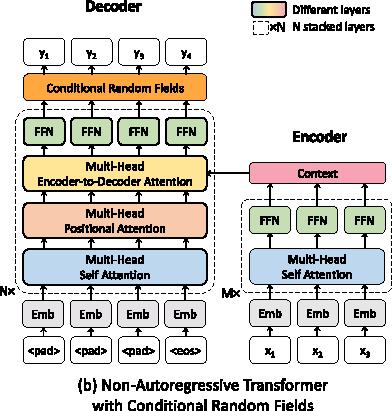
\includegraphics[width=1.0\linewidth]{./figure/Figure1_b.pdf}
\end{center}
\end{column}
\end{columns}
\end{frame}

\begin{frame}[label={sec:orge07e6cc}]{Conditional random field}
\begin{itemize}
\item Non-Autoregressive なモデルのマルチモダリティ問題を構造化推論モジュールにより対処
\begin{itemize}
\item 出力単語をラベルとした系列ラベリング問題と見なし, CRF を用いる
\end{itemize}
\end{itemize}
\begin{equation*}
    P(y|x) = \frac{1}{Z(x)} \mathrm{exp}(\sum_{i=1}^n s(y_i, x, i) + \sum_{i=2}^n t(y_{i-1}, y_i, x, i))
\end{equation*}

\begin{center}
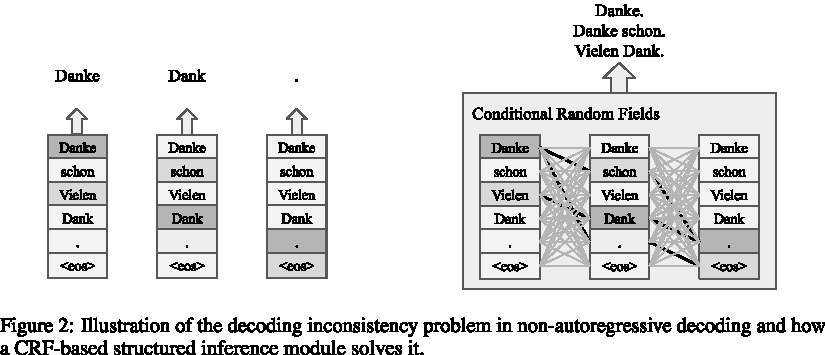
\includegraphics[width=0.9\linewidth]{./figure/Figure2.pdf}
\end{center}
\end{frame}

\begin{frame}[label={sec:orgc4097bb}]{Incorporating CRF into NART model}
\begin{equation*}
    P(y|x) = \frac{1}{Z(x)} \mathrm{exp}(\sum_{i=1}^n s(y_i, x, i) + \sum_{i=2}^n t(y_{i-1}, y_i, x, i))
\end{equation*}

\begin{itemize}
\item CRF をそのままモデルに適用すると遷移行列のサイズが \(|\mathcal{V}| \times |\mathcal{V}|\) になる
\begin{itemize}
\item 語彙数 32k のとき, 32k\(^{\text{2}}\) = 1.024B となり, 実用不可
\item 低ランク近似とビーム近似により解決
\end{itemize}
\end{itemize}
\end{frame}

\begin{frame}[label={sec:org5835aa8}]{\large Low-rank approximation for transition matrix}
\begin{itemize}
\item 遷移行列 \(M\) を低ランクな行列の積で表現
\end{itemize}

\begin{align*}
    M &= E_1 E_2^\top & \mathrm{where} & E_1, E_2 \in \mathbb{R}^{|\mathcal{V}|\times d_t}
\end{align*}
\begin{itemize}
\item 分配関数 \(Z(x)\) ・ビタビ復号以外の計算効率化
\end{itemize}
\end{frame}

\begin{frame}[label={sec:org4efdd26}]{Beam approximation for CRF}
\begin{itemize}
\item 分配関数 \(Z(x)\) ・ビタビ復号時の計算に使用
\item 各位置でk-bestを求める
\begin{itemize}
\item 分配関数 \(Z(x)\) に正解文の系列を含ませて計算
\end{itemize}
\item k-best遷移行列を用いて計算( \(|\mathcal{V}|\times|\mathcal{V}| \rightarrow k \times k\) )

\item 低ランク近似とビーム近似によりCRFの計算量は \(O(|\mathcal{V}|^2) \rightarrow O(nk^2)\)
\end{itemize}
\end{frame}

\begin{frame}[label={sec:org7c3a053}]{Dynamic CRF transition}
\begin{itemize}
\item 遷移行列 \(M\) は一系列に対して固定
\item 位置 \(i\) ごとに変化する動的な遷移行列 \(M^i\) を定義
\end{itemize}
\begin{align*}
    M_{dynamic}^{i} = f([h_{i-1}, h_i]) \\
    M^i = E_1 M_{dynamic}^i E_2^\top \\
    t(y_{i-1}, y_i, x, i) = M_{y_{i-1}, y_i}^i
\end{align*}
※ \(f: \mathbb{R}^{2d_{model}} \rightarrow \mathbb{R}^{d_t \times d_t}\) は2層のFeed Forward Network
\end{frame}

\begin{frame}[label={sec:org3c9983c}]{\large Joint training with vanilla non-autoregressive loss}
\begin{itemize}
\item モデル学習を効率的に行うため, 目的関数 \(\mathcal{L}\) はCRFの出力のNLL損失( \(\mathcal{L}_{CRF}\) )とNARTのNLL損失( \(\mathcal{L}_{NAR}\) )の荷重和とする
\end{itemize}

\begin{equation*}
    \mathcal{L} = \mathcal{L}_{CRF} + \lambda \mathcal{L}_{NAR}
\end{equation*}
※ \(\lambda\) は損失の重みをコントロールするハイパーパラメータ
\end{frame}

\begin{frame}[label={sec:org88f175b}]{Inference}
\begin{block}{目的言語文の文長 \(T^\prime\)}
\begin{description}
\item[{訓練時}] 正解文長を使用
\item[{推論時}] ソース文長 \(T\) から決定: \(T^\prime = T+C\)
\end{description}
\begin{itemize}
\item \(C\) は訓練データの文長の統計情報により決定される定数
\begin{itemize}
\item 言語ごとの文の平均長によって決定
\end{itemize}
\end{itemize}
\end{block}

\begin{block}{推論時の rescoreing}
\begin{itemize}
\item \([(T+C)-B, (T+C) + B]\) の範囲で異なるターゲット文長の翻訳候補を生成
\begin{itemize}
\item \(B\) は 4 or 9 に設定 \(\rightarrow\) 候補の数は 9 or 19 個
\end{itemize}
\item Autoregressive な Transformer を教師モデルとして最適な翻訳を選択
\end{itemize}
\end{block}
\end{frame}

\begin{frame}[label={sec:org09bcb0f}]{Experiments}
\begin{itemize}
\item データセット : WMT14 En-De/De-En, IWSLT14 De-En
\item 低ランク近似の遷移行列の埋め込み次元 : \(d_t = 32\)
\item ビーム近似のビーム幅 : \(k = 64\)
\item 目的関数 \(\mathcal{L} = \mathcal{L}_{CRF} + \lambda \mathcal{L}_{NAR}\) : \(\lambda = 0.5\)
\end{itemize}
\end{frame}

\begin{frame}[label={sec:org77f7469}]{Results}
\begin{columns}
\begin{column}{0.35\columnwidth}
\fontsize{9.5pt}{0pt}
\begin{itemize}
\item 既存の Non-autoregressive モデルより大幅に性能改善
\item WMTのEn-Deにおいて, 強力なAutoregressiveモデル(LSTM-base, CNN-base)よりも優れた性能
\item ARTとNARTの性能差(BLEU)を0.61まで縮めた
\item latencyについて, NART-CRF/DCRFは, rescoreringなしで 11.1/10.4, rescoreringありでも4.45/4.39  倍の速度向上
\end{itemize}
\end{column}


\begin{column}{0.65\columnwidth}
\begin{center}
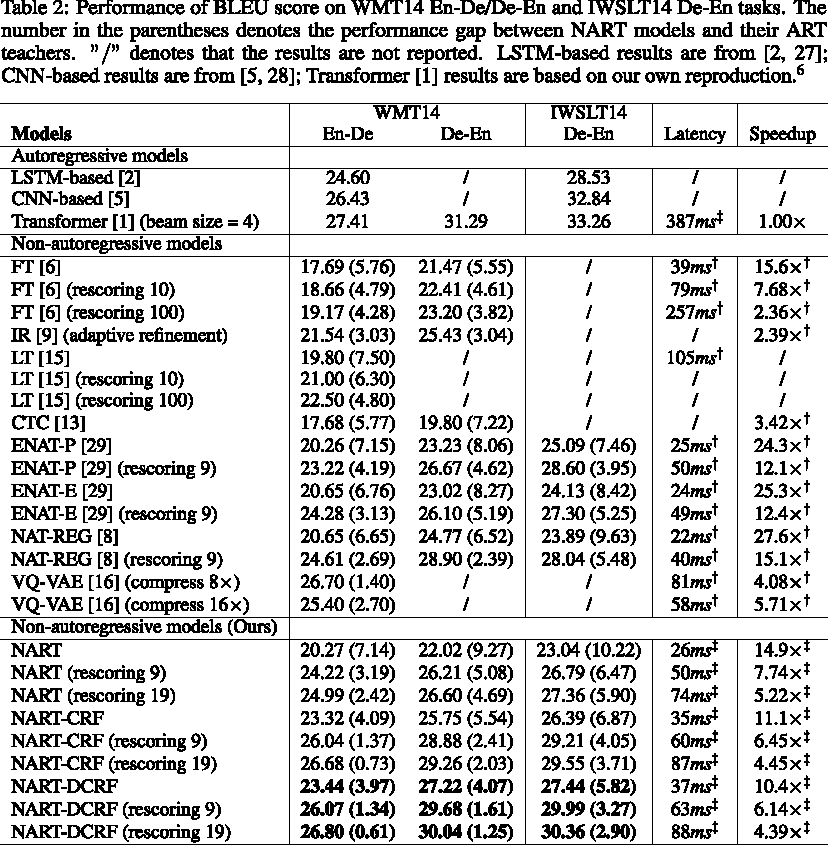
\includegraphics[width=1.0\linewidth]{./figure/Table2.pdf}
\end{center}
\end{column}
\end{columns}
\end{frame}

\begin{frame}[label={sec:orgadd54d4}]{Analysis}
\begin{itemize}
\item Dynamic CRFの効果は, En-Deでは小さく, De-Enで大きい
\begin{itemize}
\item 言語間の特性が原因
\end{itemize}
\item ビーム近似の有効性
\begin{itemize}
\item 完全な遷移行列にどれほど適合するか?
\item ビーム近似のビーム幅を64, 評価時のビーム幅 \(k\) を変えて実験
\begin{itemize}
\item \(k = 16\) 以降の上がり幅は小さい
\item 訓練時のビーム幅よりも小さい \(k = 16\) の時点ですでに良く近似できている
\end{itemize}
\end{itemize}
\end{itemize}
\end{frame}

\begin{frame}[label={sec:org549a0e8}]{Conclusion and Future Work}
\footnotesize

Conclusion
\begin{itemize}
\item Non-autoregressive なモデルのマルチモダリティ問題を解決するため, linear-chain CRFを導入し, 単語間の共起関係を扱えるようにした
\item 計算量が語彙数に依存しない, 低ランク近似, ビーム近似を提案
\item 位置毎のコンテキストをモデル化するDynamic CRFを提案
\end{itemize}

Future Work
\begin{itemize}
\item Autoregressiveモデルとのギャップを埋める
\item rescoring の処理によってlatencyが増加している
\begin{itemize}
\item 目的言語文の文長を予測するモジュールが役立つかもしれない
\end{itemize}
\end{itemize}
\begin{center}
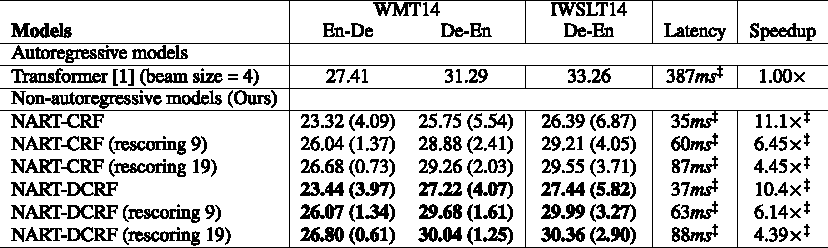
\includegraphics[width=0.8\linewidth]{./figure/Table2_art_nart.pdf}
\end{center}
\end{frame}
\end{document}
